\normaltrue
\correctionfalse

%\UPSTIidClasse{12} % 11 sup, 12 spé
%\newcommand{\UPSTIidClasse}{11}

\exer{Mouvement T $\star$ \label{C2:07:01}}
\setcounter{numques}{0}
\UPSTIcompetence[2]{C2-07}
\index{Compétence C2-07}
\index{Principe fondamental de la statique}
\index{PFS}
\index{Mécanisme à 1 translation}
\ifcorrection
\else
\textbf{Pas de corrigé pour cet exercice.}
\fi


Soit le mécanisme suivant. On note $\vect{AB}=\lambda(t)\vect{i_0}$. On note $m_1$ la masse du solide \textbf{1}.
On note $G$ le centre d'inertie de \textbf{1} tel que $\vect{BG}=\ell \vect{j_1}$ ($\vj{1}=\vj{0}$). La pesanteur est telle que $\vect{g}=-g\vect{i_0}$. Un vérin pneumatique positionné entre \textbf{1} et \textbf{0} permet de maintenir \textbf{1} en équilibre. 
%On souhaite prendre en compte les frottements secs dans la liaison glissière.
%M et $\inertie{B}{1}=\matinertie{A_1}{B_1}{C_1}{-D_1}{0}{0}{\bas{1}}$.
\begin{center}
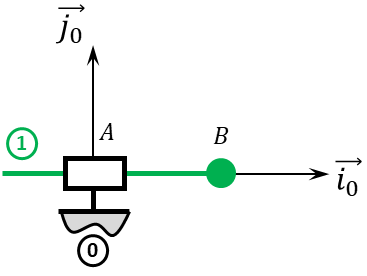
\includegraphics[width=.6\linewidth]{01_T_01}
\end{center}


On donne 
%$\torseurstat{F}{0}{1}=\torseurl{Y_{01}\vj{1}+Z_{01}\vk{1}}{L_{01}\vi{1}+M_{01}\vj{1}+N_{01}\vk{1}}{A}$,
$\torseurstat{F}{\text{pes}}{1}=\torseurl{-m_1g\vi{1}}{\vect{0}}{G}$ et 
$\torseurstat{F}{\text{ver}}{1}=\torseurl{F_v\vi{1}}{\vect{0}}{A}$.

\question{Réaliser le graphe d'analyse en faisant apparaître l'ensemble des actions mécaniques.}
\ifprof
\begin{center}
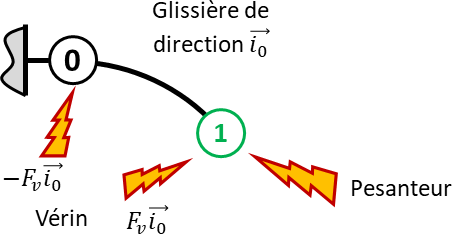
\includegraphics[width=.35\linewidth]{01_T_01_c}
\end{center}
\else
\fi


On isole \textbf{1} et on applique le théorème de la résultante statique en projection suivant $\vi{0}$.

\question{Exprimer l'équation d'équilibre de la pièce~\textbf{1}.}
\ifprof
\begin{itemize}
\item On isole \textbf{1}.
\item Bilan des actions mécaniques :
\begin{itemize}
\item pesanteur : $\torseurstat{F}{\text{pes}}{1}=\torseurl{-m_1g\vi{1}}{\vect{0}}{G}$;
\item vérin : $\torseurstat{F}{\text{ver}}{1}=\torseurl{F_v\vi{1}}{\vect{0}}{A}$;
\item liason glissière : $\torseurstat{F}{0}{1}=\torseurl{Y_{01}\vj{1}+Z_{01}\vj{1}}{L_{01}\vi{1}+M_{01}\vj{1}+N_{01}\vj{1}}{A}$.
\end{itemize}
En appliquant le théorème de la résultante statique en projection suivant $\vi{0}$, on a $-m_1g+F_v = 0$/ 

\end{itemize}
\else
\fi

\question{Déterminer l'ensemble des inconnues de liaison.}
\ifprof
\else
\fi



\ifprof
\else
%\footnotesize
%\begin{center}
%\begin{tabular}{|p{.9\linewidth}|}
%\hline
%Indications :
%\begin{enumerate}
%\item .
%\end{enumerate} \\ \hline
%\end{tabular}
%\end{center}
%\normalsize

\begin{flushright}
\footnotesize{Corrigé  voir \ref{C2:07:01}.}
\end{flushright}%
\fi


